\begin{enumerate}
\item If the angle between two tangents drawn from an external point P to a circle of radius a and centre O, $60\degree$is then find the length of OP.
\item Prove that the lengths of two tangents drawn from an external point to a circle are equal.
\item Prove that the tangents drawn at the end points of a chord of a circle makes equal angles with the chord.
\item A circle touches all the four sides of a quadrilateral $ABCD$. Prove that 
 \begin{align*}
        AB + CD = BC + DA
 \end{align*}
\item In the given figure, $XY$ and $X\rq Y\rq$ are two parallel tangents to a circle with centre $O$ and another tangent $AB$ with point of contact $C$, is intersecting $XY$ at $A$ and $X\rq Y\rq$ at $B$. Prove that $\angle{AOB}$=90$\degree$.
\begin{figure}[H]
\centering
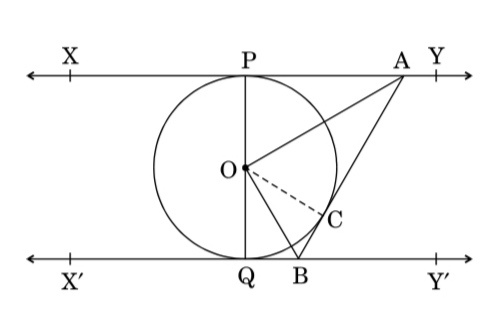
\includegraphics[width=0.8 \columnwidth]{figs/cir1.jpg}
\end{figure}
\end{enumerate}
